\section{Experiments }
\label{sec:Experiments}

\subsection{Experiment Setup}
\begin{table}[t!]
    \centering
    \setlength{\tabcolsep}{4pt}
    \resizebox{\columnwidth}{!}{%
    \begin{tabular}{c|l|cccc}
        % \toprule
        \topline
        %
        
       \rowcolor{mygray} 
       
       &  Method   & {HOTA}$\uparrow$ & {OSPA}$\downarrow$ & {IDF1}$\uparrow$ & {MOTA} $\uparrow$  \\
        % \midrule 
        \hline
        

       \parbox[t]{3mm}{\multirow{3}{*}{\rotatebox[origin=c]{90}{E2E}}} & TrackFormer~\cite{meinhardt2021trackformer} &  19.16 &  0.95  & 19.66 & 17.79  \\
        & MOTRv2~\cite{zhang2023motrv2}   &  18.22 & \textbf{0.93}  & 19.30 & 12.30  \\
        %
        & \cellcolor{tabgray}\name{}$_{E2E}$ \text{(ours)} & \cellcolor{tabgray}\textbf{21.56} & \cellcolor{tabgray}0.94 & \cellcolor{tabgray}\textbf{22.87} & \cellcolor{tabgray}\textbf{25.01} \\

        
        % \midrule
        \hline
        \parbox[t]{3mm}{\multirow{8}{*}{\rotatebox[origin=c]{90}{TBD}}} 
        & SORT~\cite{bewley2016simple}    &  23.49 & 0.90  & 26.11 & 24.59  \\
        & DeepSORT~\cite{wojke2017simple}  &  22.15 &  0.95 & 23.46 & 24.88 \\
        & ByteTrack~\cite{zhang2022bytetrack}   &   25.00 &  0.86  & 27.95 & 26.59 \\
        & Bot-SORT~\cite{aharon2022bot} &    22.90  & 0.91  & 24.27 & 23.08  \\
        & OC-SORT~\cite{cao2023observation} &     25.04 & \textbf{0.84}  & 27.89 & 25.64  \\
        & HybridSORT~\cite{yang2024hybrid}  &  25.01  &  0.85 & 27.82  & 25.03  \\
        & DiffMOT~\cite{lv2024diffmot} &    19.96  & 0.95  & 20.26 &  20.05  \\
        %
        & \cellcolor{tabgray}\name{}$_{DA}$ \text{(ours)} & \cellcolor{tabgray}\textbf{26.92} & \cellcolor{tabgray}\textbf{0.84} & \cellcolor{tabgray}\textbf{30.26} & \cellcolor{tabgray}\textbf{26.60}  \\
        % \bottomrule
        \bottomline
    \end{tabular}
    }
    \vspace{-1ex}
    \caption{Comparison with state-of-the-art methods on the JRDB test set~\cite{martin2021jrdb}.}
    \vspace{-2ex}
    \label{tab:sota JRDB}
\end{table}
\vspace{ 1 ex}
\begin{table}[t!]
    \centering
    \setlength{\tabcolsep}{4pt}
    \resizebox{\columnwidth}{!}{%
    \begin{tabular}{c|l|cccc}
        % \toprule
        \topline
        %

        \rowcolor{mygray} &  Method  & {HOTA}$\uparrow$ & {OSPA}$\downarrow$ & {IDF1}$\uparrow$ & {MOTA} $\uparrow$  \\
        % \midrule 
        \hline
        

       \parbox[t]{3mm}{\multirow{3}{*}{\rotatebox[origin=c]{90}{E2E}}} & TrackFormer~\cite{meinhardt2021trackformer} &  19.62 & 0.97  & 17.75 &  \textbf{3.16}  \\
        & MOTRv2~\cite{zhang2023motrv2}    & 16.42 & \textbf{0.96}   & 17.08  & -0.06\\
        %
        & \cellcolor{tabgray}\name{}$_{E2E}$ \text{(ours)} & \cellcolor{tabgray}\textbf{19.87} & \cellcolor{tabgray}0.98 & \cellcolor{tabgray}\textbf{19.47} & \cellcolor{tabgray}-5.89  \\

 	 	 	 
         	 	 	 
	 	  	 	 	 

        % \midrule  	 	 	 

        \hline
        \parbox[t]{3mm}{\multirow{8}{*}{\rotatebox[origin=c]{90}{TBD}}} 
        & SORT~\cite{bewley2016simple}    & 14.57  & 0.98  & 15.60 & 4.81  \\
        & DeepSORT~\cite{wojke2017simple} & 21.16  & 0.96  & 22.56 & 5.12  \\
        & ByteTrack~\cite{zhang2022bytetrack}   & 20.66  & \textbf{0.94}  & 22.56 & 8.68  \\
        & Bot-SORT~\cite{aharon2022bot} & 15.77  & 0.99  & 15.65 & 5.92  \\
        & OC-SORT~\cite{cao2023observation}&  20.83 & \textbf{0.94} & 22.60 & 7.65  \\ 	 	 	
        & HybridSORT~\cite{yang2024hybrid}  &  16.64  & 0.96  & 17.38 & 6.79  \\
        & DiffMOT~\cite{lv2024diffmot} &  16.40 & 0.97  & 16.62 & 6.21 \\ 	 	 	 

        %
        & \cellcolor{tabgray}\name{}$_{DA}$ \text{(ours)} & \cellcolor{tabgray}\textbf{23.45} & \cellcolor{tabgray}\textbf{0.94} & \cellcolor{tabgray}\textbf{26.41} & \cellcolor{tabgray}\textbf{9.68} \\

        % \bottomrule
        \bottomline
    \end{tabular}
    } 	 	 	 
	 	 	 

    \vspace{-1ex}
    \caption{Comparison with state-of-the-art methods on the QuadTrack test set.}
    \vspace{-3mm}
    \label{tab:sota QaudTrack}
\end{table}

%
%



\begin{table*}[t!]
    \centering
    \setlength{\tabcolsep}{4pt}
    \resizebox{2\columnwidth}{!}{%
    \begin{tabular}{c|l|l|ll|lllll}
        % \toprule
        \topline
          \rowcolor{mygray} & Association Method & Detection Method& HOTA $ \uparrow$ & IDF1$\uparrow$ & OSPA $\downarrow$  & MOTA$\uparrow$ & DetA $\uparrow$ & AssA $\uparrow$ & FPS $\uparrow$ \\
         % \midrule
         \hline
        \parbox[t]{3mm}{\multirow{12}{*}{\rotatebox[origin=c]{90}{Track-By- Detection (TBD)}}} 
         %
         & \multirow{3}{*}{SORT~\cite{bewley2016simple}} & YOLO11~\cite{yolo11} (baseline) & 25.83 & 29.56 & 0.915 & 31.02 & 27.62 & 24.51  & 49.18\\
         
         &  & OmniTrack$_{Det}$~\text{(ours)} & 26.34 \textcolor{codegreen}{(+0.51)} & 31.11 \textcolor{codegreen}{(+1.55)} & 0.907 \textcolor{codegreen}{(-0.008)} & 34.21 \textcolor{codegreen}{(+3.19)} & 30.52 \textcolor{codegreen}{(+2.90)} & 22.96 \textcolor{black}{(-1.55)} & 12.14 \\

        
        
        &  & OmniTrack$_{DA}$~\text{(ours)} & 29.44 \textcolor{codegreen}{(+3.10)} & 33.27 \textcolor{codegreen}{(+2.16)} & 0.927\textcolor{black}{(+0.020)} & 33.44 \textcolor{black}{(-0.77)} & 35.16 \textcolor{codegreen}{(+4.64)} & 25.06 \textcolor{codegreen}{(+2.10)} & 11.78\\
         \cline{2-10}
         % \cmidrule{2-9}

        & \multirow{3}{*}{ByteTrack~\cite{zhang2022bytetrack}} & YOLO11~\cite{yolo11} (baseline) & 27.85 & 32.20 & 0.896 & 34.46 & 31.49 & 25.15 & 50.36\\
         &  & OmniTrack$_{Det}$\text{(ours)} & 28.14 \textcolor{codegreen}{(+0.29)} & 32.97 \textcolor{codegreen}{(+0.77)} & 0.870 \textcolor{codegreen}{(-0.026)} & 37.36 \textcolor{codegreen}{(+2.90)} & 32.94 \textcolor{codegreen}{(+1.45)} & 24.29 \textcolor{black}{(-0.86)} & 12.24\\
         &  & OmniTrack$_{DA}$~\text{(ours)} & 29.58 \textcolor{codegreen}{(+1.44)} & 34.54 \textcolor{codegreen}{(+1.57)} & 0.859 \textcolor{codegreen}{(-0.011)} & 38.14 \textcolor{codegreen}{(+0.78)} & 34.71 \textcolor{codegreen}{(+1.77)} & 25.49 \textcolor{codegreen}{(+1.20)} & 11.83\\
         % \cline{2-11}
         % \cmidrule{2-9}
         \cline{2-10}


         
        

        & \multirow{3}{*}{OC-SORT~\cite{cao2023observation}} & YOLO11~\cite{yolo11} (baseline) & 29.26 & 33.69 & 0.874 & 34.22 & 31.81 & 27.48 & 46.33\\
         &  & OmniTrack$_{Det}$~\text{(ours)} & 29.43 \textcolor{codegreen}{(+0.17)} & 34.11 \textcolor{codegreen}{(+0.42)} & 0.851 \textcolor{codegreen}{(-0.023)} & 38.72 \textcolor{codegreen}{(+4.50)} & 34.48 \textcolor{codegreen}{(+2.67)} & 25.39 \textcolor{black}{(-2.09)} & 11.59\\
         &  & OmniTrack$_{DA}$~\text{(ours)} & 30.65 \textcolor{codegreen}{(+1.22)} & 34.83 \textcolor{codegreen}{(+0.72)} & 0.838 \textcolor{codegreen}{(-0.013)} & 36.37 \textcolor{black}{(-2.35)} & 35.58 \textcolor{codegreen}{(+1.10)} & 26.76 \textcolor{codegreen}{(+1.37)} & 11.13\\
         % \cline{2-11}
         % \cmidrule{2-9}
         \cline{2-10}



        

        & \multirow{3}{*}{HybridSORT~\cite{yang2024hybrid}} & YOLO11~\cite{yolo11} (baseline) & 29.71 & 34.16 & 0.877 & 34.71 & 31.70 & 28.39 & 44.34\\
         &  & OmniTrack$_{Det}$~\text{(ours)} & 30.00 \textcolor{codegreen}{(+0.29)} & 34.09 \textcolor{black}{(-0.07)} & 0.853 \textcolor{codegreen}{(-0.024)} & 32.32 \textcolor{black}{(-2.39)} & 35.02 \textcolor{codegreen}{(+3.32)} & 26.09 \textcolor{black}{(-2.30)} & 11.65\\
         &  & OmniTrack$_{DA}$~\text{(ours)} & 31.05 \textcolor{codegreen}{(+1.05)} & 36.06 \textcolor{codegreen}{(+1.97)} & 0.850 \textcolor{codegreen}{(-0.003)} & 38.13 \textcolor{codegreen}{(+5.81)} & 35.08 \textcolor{codegreen}{(+0.06)} & 27.78 \textcolor{codegreen}{(+1.69)} & 10.96\\
         % \cline{2-11}
         % \cmidrule{2-11}
         

    
         \hline
         \hline
         	 	 	 	 	 

         \parbox[t]{3mm}{\multirow{4}{*}{\rotatebox[origin=c]{90}{ E2E}}} 
         %
         & TrackFormer~\cite{meinhardt2021trackformer} & \multicolumn{1}{c|}{\centering\textit{n.a.}}  & 22.22 & 23.38 & 0.959 & 23.83 & 30.30 & 16.93 & 7.38\\
         & MOTR~\cite{zeng2022motr} & \multicolumn{1}{c|}{\centering\textit{n.a.}} & 19.78 & 23.25 & 0.928 & 25.44  & 25.51 & 15.61 & 12.73\\
         & MOTRv2~\cite{zhang2023motrv2} & \multicolumn{1}{c|}{\centering\textit{n.a.}} & 24.68 & 25.49 & \textbf{0.911} & 17.05 & 26.83 & 22.97 & \textbf{13.01}\\
         &   \name{}$_{E2E}$~\text{(ours)} &  \multicolumn{1}{c|}{\centering\textit{n.a.}}  & \textbf{25.12} & \textbf{27.42} & 0.925 & \textbf{34.99} & \textbf{33.35} & \textbf{19.17}  & 11.64\\
         % \bottomrule
         \bottomline
    \end{tabular}
    }        
        
    \caption{Results on the JRDB validation set~\cite{martin2021jrdb}. The first four groups compare methods under the TBD paradigm, whereas the last group presents a comparison under the E2E paradigm. In the TBD paradigm, each method is evaluated under three detection methods: the baseline with YOLO11 \cite{yolo11} as the detector, the OmniTrack$_{Det}$ detector, and OmniTrack$_{DA}$. The \textcolor{codegreen}{numbers} represent the improvement relative to the previous line's method. The FPS metric is measured on a single RTX 3090 GPU with an image resolution of $4160\times480$.
    %
    }
    \vspace{-3mm}
    \label{tab:baseline}
\end{table*}
\begin{table}[t!]
    \centering
    \setlength{\tabcolsep}{8pt}     % 4pt
    \resizebox{\columnwidth}{!}{%
    \begin{tabular}{c|cc|cccc}
        % \toprule
        \topline
        \rowcolor{mygray}  Exp. & \textit{I$_{dn}$} & \textit{I$_{ft}$} & HOTA$\uparrow$ & IDF1$\uparrow$ & OSPA$\downarrow$ & MOTA$\uparrow$ \\
        % \midrule
        \hline
        
        \ding{192} & - & - &  0.01 & 0.00 & 1.00 & 0.00  \\ 	 	 	 

        \ding{193} & & \checkmark   & 3.80 & 1.91 & 0.99 & -0.01 \\
        \ding{194} &   \checkmark  & & 24.32 & 26.20 &0.93  & 29.25     \\ 	 	 	

        % \midrule
        \hline
        \rowcolor{tabgray}\ding{195} & \checkmark & \checkmark  & \textbf{25.12} & \textbf{27.42} & \textbf{0.93} & \textbf{34.99}  \\
        % \bottomrule
        \bottomline
    \end{tabular}
    }
    \vspace{-1mm}
    \caption{Analysis of FlexiTrack Instance: \(\textit{I}_{dn}\) represents an instance generated using Ground Truth (GT), whereas \(\textit{I}_{ft}\) refers to a FlexiTrack Instance.
    }
    \vspace{-3mm}
    \label{tab: FlexiTrack_instance.}
\end{table}





\paragraph{Datasets.}
We conduct experiments on two datasets: JRDB~\cite{martin2021jrdb} and QuadTrack. 
JRDB is a panoramic dataset designed for crowded human environments, comprising $10$ training sequences, $7$ validation sequences, and $27$ test sequences.
The panoramic images in this dataset are stitched using a wheeled mobile robot equipped with five pinhole cameras. It includes both outdoor and indoor scenes, characterized by significant occlusion and the presence of small objects. 
Additionally, some objects exhibit rapid relative motion to the robot, which presents substantial challenges for MOT algorithms. Detailed information regarding the QuadTrack dataset is elaborated in Sec.~\ref{sec:QuadTrack}.

\vspace{-3mm}
\paragraph{Metrics.}
%
We employ the CLEAR metrics~\cite{bernardin2008evaluating}, including MOTA, DetA, and AssA, alongside IDF1~\cite{ristani2016performance}, OPSA~\cite{martin2021jrdb}, and HOTA~\cite{luiten2021hota} for a comprehensive tracking performance evaluation. MOTA is primarily influenced by detector performance, IDF1 measures identity preservation, and HOTA integrates association and localization accuracy, making it increasingly pivotal for tracking assessment.

\vspace{-3mm}
\paragraph{Implementation details.}
To enable a fair comparison of various MOT algorithms, we retrained models on the JRDB dataset. 
For End-To-End (E2E) algorithms~\cite{zhang2023motrv2,meinhardt2021trackformer,zeng2022motr}, we trained using the default parameters from the source code on JRDB. 
For the MOT algorithms~\cite{zhang2022bytetrack,cao2023observation,bewley2016simple,yang2024hybrid} based on the TBD paradigm, we selected the advanced YOLO11-X \cite{yolo11} as the baseline detector for training on JRDB. Additionally, OmniTrack$_{Det}$ was obtained by masking the Track Management module after training the OmniTrack model and saving the detection results. The AdamW optimizer~\cite{kingma2014adam} was used, with the learning rate set to \(10^{-5}\). For additional experimental details, please refer to the supplementary. 
%

\subsection{Comparison with State of the Art}
\paragraph{Tracking on JRDB test set.} 
In Tab.~\ref{tab:sota JRDB}, we compare our OmniTrack with state-of-the-art methods on the JRDB test set. Firstly, our approach significantly outperforms existing algorithms across all tracking metrics, whether in comparison with End-to-End or TBD paradigms. Specifically, OmniTrack achieves an impressive HOTA of $21.56\%$ and an IDF1 of $22.87\%$ within the End-to-End framework, surpassing the current state-of-the-art method, MOTRv2~\cite{zhang2023motrv2}, by $3.34\%$ and $3.57\%$, respectively. Furthermore, in the TBD paradigm, even under the same detector conditions, OmniTrack outperforms the state-of-the-art HybridSORT~\cite{yang2024hybrid} by $1.91\%$ in HOTA and $2.44\%$ in IDF1, demonstrating its superior performance.

\vspace{-3mm}
\paragraph{Tracking on QuadTrack test set.}
%

In Tab.~\ref{tab:sota QaudTrack}, we present a comparison between OmniTrack and state-of-the-art methods on the QuadTrack test set. This dataset is particularly challenging, characterized by a panoramic FoV and rapid, non-linear sensor motion, which introduces significant complexities for traditional MOT algorithms. Despite these challenges, our method outperforms existing approaches, achieving the highest HOTA scores: $19.87\%$ for the E2E group and $23.45\%$ for the TBD group. 
%

\subsection{Paradigm Comparison}
\paragraph{Baseline.}
To further validate the advantages of OmniTrack, we conducted comparisons based on the TBD and E2E paradigms, as shown in Tab.~\ref{tab:baseline}.
In the TBD paradigm, we evaluated several baseline tracking algorithms \cite{bewley2016simple,zhang2022bytetrack,cao2023observation,yang2024hybrid}. Each tracking method was compared under three different detection setups: using YOLO11-X~\cite{yolo11} as the baseline detector, OmniTrack\(_{Det}\) as the detector (representing traditional TBD tracking where detection and tracking are independent), and OmniTrack\(_{DA}\) with a feedback mechanism for TBD tracking. In the E2E paradigm, we used MOTR~\cite{zeng2022motr} as the baseline for comparison.

\vspace{-3mm}
\paragraph{Result.}
In the TBD method, {OmniTrack\(_{Det}\)} consistently outperforms {YOLO11-X}~\cite{yolo11}, showing an average improvement of $0.2\%$ in HOTA and $0.6\%$ in IDF1. Despite {OmniTrack\(_{Det}\)} not having a speed advantage, it achieves notable improvements in accuracy. Furthermore, when comparing {OmniTrack\(_{Det}\)} to {OmniTrack\(_{DA}\)}, the latter shows an average increase of $1.7\%$ in HOTA and $1.4\%$ in IDF1, demonstrating the effectiveness of the feedback mechanism. In the E2E paradigm, {OmniTrack\(_{E2E}\)} achieved the best result HOTA of $25.12\%$ and IDF1 of $27.42\%$.

%

\subsection{Ablation Study}

\paragraph{Analysis of the FlexiTrack instance.}
Tab.~\ref{tab: FlexiTrack_instance.} compares experiments with and without denoise instances and FlexiTrack instances during the training phase. Experiments \ding{192} and \ding{193} demonstrate that FlexiTrack Instances are crucial for achieving the tracking objective. In Experiment \ding{194}, we observe that denoise instances, generated from Ground Truth (GT), significantly improve the HOTA score by providing stronger guidance. 
Experiments \ding{194} and \ding{195} further show that incorporating FlexiTrack instances after using denoise instances leads to a further improvement in the HOTA score.

\begin{table}[t!]
    \centering
    \setlength{\tabcolsep}{8pt}     % 4pt
    \resizebox{\columnwidth}{!}{%
    \begin{tabular}{c|ccc|ccc}
        % \toprule
        \topline
        %
        \rowcolor{mygray}  Exp. & $\mathcal{S}_5$ & $\mathcal{S}_4$ & $\mathcal{S}_3$ & HOTA$\uparrow$ & IDF1$\uparrow$ & OSPA$\downarrow$ \\
        % \midrule 
        \hline
        \ding{192} & - &  -  &  -  & 23.296 & 25.496 &0.93415\\
        \ding{193} & MLP &  MLP  &  MLP  & 21.951   & 23.535   & 0.92151 \\
        
        \ding{194} & Conv &  Conv  &  Conv  & 23.565  & 25.814  & \textbf{0.90931}\\
         	 	 	 

        \ding{195} & \checkmark &   \checkmark &  \checkmark  & 24.724 & 26.886 & 0.91934 \\
        \ding{196} &  \checkmark  &    &    & 24.426 & 26.016 &0.92819  \\
        \ding{197} &   &   & \checkmark  & 24.539 & 26.506 & 0.92776  \\
        % \midrule
        \hline
        \rowcolor{tabgray}\ding{198} &  & \checkmark &    & \textbf{25.120} & \textbf{27.423} & 0.92512  \\
        % \bottomrule
        \bottomline
    \end{tabular}
    }
    \vspace{-1mm}
    \caption{Ablation study on the CircularStatE module. $S_3$, $S_4$, and $S_5$ represent multi-scale features extracted from the backbone~\cite{He_2016_CVPR}. \emph{MLP} refers to fully connected layers, \emph{Conv} to convolutional layers. The symbol $\checkmark$ indicates the use of \emph{DynamicSSM} \ref{mod:DynamicSSM}}

    \vspace{-3mm}
    \label{tab:CSEM}
\end{table}

\vspace{-3mm}
\paragraph{Analysis of the CircularStatE module.}
In Tab.~\ref{tab:CSEM}, we evaluate the effectiveness of \emph{DynamicSSM} in the \emph{CircularStatE}, comparing it with other common designs such as Conv and MLP. 
The results from experiments \ding{193}, \ding{194}, and \ding{195} demonstrate a clear advantage for {DynamicSSM}. Experiments~\ding{196}, \ding{197}, and \ding{198} further show that applying {DynamicSSM} to $S_4$ yields the best performance. where $S_5$, $S_4$, and $S_3$ impact MOT results. Since $S_4$ contains both high-level semantic and low-level geometric features, its effect is the most pronounced.

%

\vspace{-3mm}
\paragraph{Analysis of the initialization and update thresholds.}
%

In OmniTrack\(_{E2E}\), we analyzed the impact of the \emph{initial threshold} and \emph{updated threshold} on tracking performance. As shown in Fig.~\ref{fig: thresholds}, both the \emph{initial threshold} and \emph{updated threshold} achieved HOTA scores exceeding $25\%$ within the range of $0.1$ to $0.7$. This demonstrates that OmniTrack\(_{E2E}\) is robust to threshold variations, eliminating the need for fine-tuning to achieve optimal results. 
%

\vspace{-3mm}
\paragraph{Comparison of end-to-end model training.}
\begin{table}[t!]
    \centering
    \setlength{\tabcolsep}{4pt}
    \resizebox{\columnwidth}{!}{
    \begin{tabular}{l|cccc}
        % \toprule
        \topline
        \rowcolor{mygray}  Method  & {\#Params} & {FLOPs}& {MACs}  & {Training Time} $\downarrow$   \\
        % \midrule
        \hline
        TrackFormer~\cite{meinhardt2021trackformer}   & 44.01M  & 335G   & 167G & 108 hours \\
        MOTR~\cite{zeng2022motr}  &   43.91M &  1421G & 709G &  80 hours \\
        MOTRv2~\cite{zhang2023motrv2} &  41.65M &   1395G  &  696G  &  130 hours\\
        \hline

        \rowcolor{tabgray} \name{}$_{E2E}$~\text{(ours)}    & 63.13M  &  762G   & 369G & 20 hours\\

        % \bottomrule
        \bottomline
    \end{tabular}
    }
    \vspace{-1mm}
    \caption{Comparison of parameters, FLOPs, MACs, and training time for various end-to-end models on the JRDB dataset~\cite{martin2021jrdb}.}
    \vspace{-3mm}
    \label{tab:6_para}
\end{table}

%
In Tab.~\ref{tab:6_para}, we compare the number of parameters and training time of OmniTrack\(_{E2E}\) with existing End-to-End methods. 
Our method trains over four times faster than other End-to-End methods using default parameters on the JRDB dataset. 
This is achieved by implementing identity association through FlexiTrack Instances, which significantly simplifies the model design of the association component and alleviates the challenges associated with E2E model training.

\begin{figure}[!t]
  \centering
  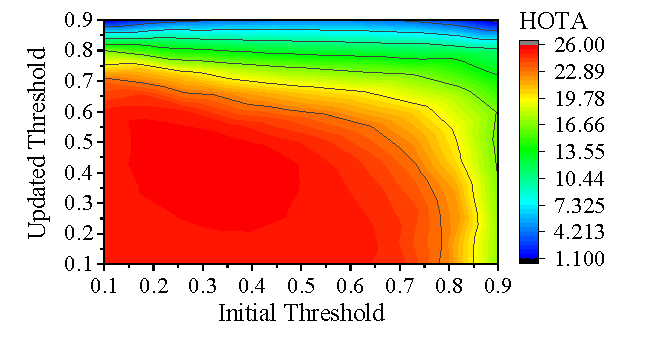
\includegraphics[width=0.48\textwidth]{imgs/HOTA.pdf}
  \vskip-3ex
  \caption{Effects of the trajectory initialization threshold and update threshold on the HOTA metric in OmniTrack$_{E2E}$.}
  \label{fig: thresholds}
  \vskip -4ex
\end{figure}
